% -*- coding: utf-8 -*-
\documentclass[9pt]{beamer}

\usetheme[secheader]{Boadilla}
%\usepackage[french]{babel}
% use utf8 because bug with package circuitikz
\usepackage[utf8]{inputenc}

\usepackage{hyperref}
\usepackage{graphicx}
\usepackage{media9}
\usepackage{amsmath,amsthm,amsfonts}
%\usepackage{theorem}

\title{}
\begin{document}

\begin{frame}{}
  \maketitle
\end{frame}

\section{Problem statement}

\begin{frame}{Eye description}
Eye is the organs of vision; it allows the conversion of light into impulses in neurons
\begin{center}
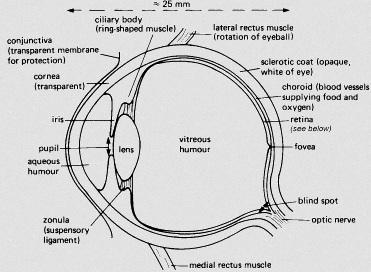
\includegraphics[width=.7\linewidth]{Eye.jpg}
\end{center}
\tiny{source: \url{http://academia.hixie.ch/bath/eye/home.html}}
\end{frame}

\begin{frame}{Eye description}
\begin{center}
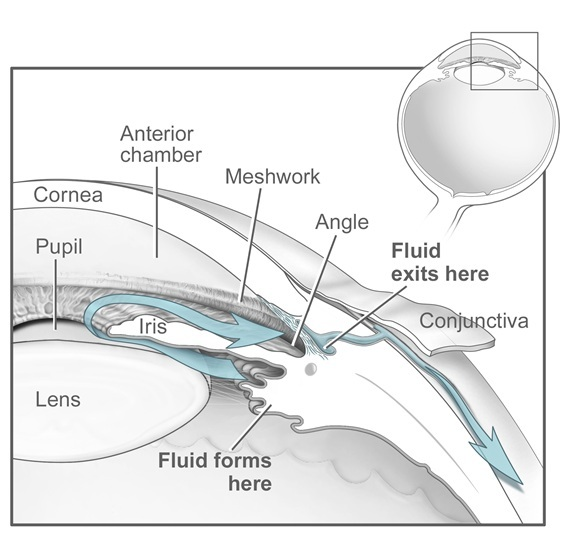
\includegraphics[width=.5\linewidth]{Humor.jpg}
\end{center}
Aqueous humor is produced by the ciliary epithelium and drains into the Schlemm's canal and the pressure produced is the intra-ocular pression.


\end{frame}

\begin{frame}{IOP measure:tonometry}

\end{frame}

\begin{frame}{Glaucoma}

\end{frame}

\begin{frame}{Treatment}

\end{frame}

\section{Mathematical Model}

\begin{frame}{Mass balances}

\end{frame}

\begin{frame}{Assumptions}

\end{frame}

\begin{frame}{Data}

\end{frame}

\section{Numerical Results}

\begin{frame}{Recovering some values}

\end{frame}

\end{document}



%%% Local Variables:
%%% coding: utf-8
%%% mode: latex
%%% TeX-PDF-mode: t
%%% TeX-parse-self: t
%%% x-symbol-8bits: nil
%%% TeX-auto-regexp-list: TeX-auto-full-regexp-list
%%% TeX-master: t
%%% ispell-local-dictionary: "american"
%%% End:
